


%%%%%%%%%%%%%%%%%%%%%%%%%%%%%%%%%%%%%%%%%%%%%%%%%%%%%%%%
% Dataset Analysis
%%%%%%%%%%%%%%%%%%%%%%%%%%%%%%%%%%%%%%%%%%%%%%%%%%%%%%%%
\section{Model Zoo Analysis}
\label{sec:analysis}
%
\begin{table}[]
{
\centering
\scriptsize
\caption{Analysis of the diversity of our 27 model zoos (one row per zoo). Mean (std) values in \% per zoo, computed on the last epoch. Agreement is computed using samples from the test split of the image dataset pairwise over the entire zoo. Higher agreement values indicate more uniform behavior and less behavioral diversity. Distance in weight space are computed pairwise over the entire zoo. Higher distance values indicate larger diversity in weight space.}
\label{tab:analysis}
{
\begin{center}
\centering
\begin{tabular}{@{}lllcccccc@{}}
\toprule
                               &               &               & Performance & \multicolumn{2}{c}{Agreement}    & \multicolumn{3}{c}{Weights}               \\ 
\cmidrule(rl){4-4} \cmidrule(rl){5-6} \cmidrule(rl){7-9} \\
Dataset                        & Architecture  & Config & Accuracy    & $\kappa_{aggr}$ & $\kappa_{cka}$ & $\mathbf{w}$           & l2-dist       & cos dist    \\
\cmidrule(r){1-1} \cmidrule(rl){2-2}  \cmidrule(rl){3-3} \cmidrule(rl){4-4} \cmidrule(rl){5-6} \cmidrule(rl){7-9}
\multirow{3}{*}{MNIST}         & CNN (s)   & Seed          & 91.1 (0.9)  & 88.5 (1.3)      & 77.2 (5.2)     & 18.9 (58.4) & 124.1 (4.9)   & 77.1 (4.1)  \\
                               & CNN (s)   & Hyp-10-r   & 79.9 (30.7) & 67.7 (35.5)     & 58.6 (25.9)    & 0.4 (46.5)  & 150.6 (66.5)  & 98.8 (7.2)  \\
                               & CNN (s)   & Hyp-10-f    & 80.3 (30.3) & 68.3 (35.3)     & 58.8 (25.7)    & 0.3 (46.7)  & 149.7 (66.8)  & 97.7 (10.0) \\
\cmidrule(r){1-1} \cmidrule(rl){2-2}  \cmidrule(rl){3-3} \cmidrule(rl){4-4} \cmidrule(rl){5-6} \cmidrule(rl){7-9}
\multirow{3}{*}{F-MNIST}       & CNN (s)   & Seed          & 72.7 (1.0)  & 79.8 (2.6)      & 82.3 (12.6)    & 22.6 (55.6) & 122.0 (4.9)   & 74.5 (4.4)  \\
                               & CNN (s)   & Hyp-10-r   & 68.4 (23.7) & 59.9 (29.1)     & 64.6 (23.5)    & 1.0 (46.0)  & 149.6 (62.2)  & 99.2 (6.8)  \\
                               & CNN (s)   & Hyp-10-f    & 68.7 (23.4) & 60.4 (28.7)     & 64.6 (22.7)    & 0.9 (46.3)  & 148.5 (61.9)  & 97.9 (9.9)  \\
\cmidrule(r){1-1} \cmidrule(rl){2-2}  \cmidrule(rl){3-3} \cmidrule(rl){4-4} \cmidrule(rl){5-6} \cmidrule(rl){7-9}
\multirow{3}{*}{SVHN}          & CNN (s)   & Seed          & 71.1 (8.0)  & 67.2 (10.3)     & 67.7 (15.7)    & 7.1 (113.7) & 137.6 (8.3)   & 94.5 (5.1)  \\
                               & CNN (s)   & Hyp-10-r   & 35.9 (24.3) & 61.6 (35.9)     & 17.8 (28.0)    & 1.4 (42.2)  & 170.5 (149.4) & 83.6 (30.4) \\
                               & CNN (s)   & Hyp-10-f    & 36.0 (24.4) & 61.4 (36.0)     & 18.1 (27.9)    & 1.3 (42.2)  & 170.0 (149.0) & 83.2 (30.7) \\
\cmidrule(r){1-1} \cmidrule(rl){2-2}  \cmidrule(rl){3-3} \cmidrule(rl){4-4} \cmidrule(rl){5-6} \cmidrule(rl){7-9}
\multirow{3}{*}{USPS}          & CNN (s)   & Seed          & 87.0 (1.7)  & 87.3 (2.2)      & 86.7 (6.3)     & 8.2 (26.9)  & 123.1 (5.2)   & 75.9 (5.0)  \\
                               & CNN (s)   & Hyp-10-r   & 64.7 (30.8) & 55.3 (31.4)     & 50.9 (30.5)    & 2.1 (39.6)  & 155.5 (92.6)  & 99.1 (8.9)  \\
                               & CNN (s)   & Hyp-10-f    & 65.0 (30.7) & 55.4 (31.3)     & 50.4 (30.4)    & 1.9 (40.1)  & 154.2 (93.1)  & 97.3 (13.7) \\
\cmidrule(r){1-1} \cmidrule(rl){2-2}  \cmidrule(rl){3-3} \cmidrule(rl){4-4} \cmidrule(rl){5-6} \cmidrule(rl){7-9}
\multirow{3}{*}{CIFAR10}      & CNN (s)   & Seed          & 48.7 (1.4)  & 65.7 (3.1)      & 72.9 (11.3)    & 1.1 (11.0)  & 138.7 (5.6)   & 96.3 (5.1)  \\
                               & CNN (s)   & Hyp-10-r   & 35.1 (16.3) & 33.3 (22.9)     & 47.5 (34.0)    & -0.2 (17.0) & 155.6 (71.0)  & 97.5 (10.8) \\
                               & CNN (s)   & Hyp-10-f    & 35.1 (16.2) & 33.3 (22.8)     & 47.3 (34.2)    & -0.2 (16.9) & 155.3 (70.0)  & 97.2 (11.1) \\
\cmidrule(r){1-1} \cmidrule(rl){2-2}  \cmidrule(rl){3-3} \cmidrule(rl){4-4} \cmidrule(rl){5-6} \cmidrule(rl){7-9}
\multirow{3}{*}{CIFAR10}      & CNN (m)   & Seed          & 61.5 (0.7)  & 76.0 (1.6)      & 92.4 (1.7)     & 0.1 (18.2)  & 137.0 (7.9)   & 94.1 (9.2)  \\
                               & CNN (m)   & Hyp-10-r   & 39.6 (21.8) & 34.5 (27.1)     & 43.2 (36.5)    & -0.4 (23.0) & 158.9 (79.9)  & 98.6 (12.2) \\
                               & CNN (m)   & Hyp-10-f    & 39.6 (21.7) & 34.4 (26.7)     & 42.8 (37.8)    & -0.4 (22.9) & 158.1 (77.2)  & 98.0 (13.1) \\
\cmidrule(r){1-1} \cmidrule(rl){2-2}  \cmidrule(rl){3-3} \cmidrule(rl){4-4} \cmidrule(rl){5-6} \cmidrule(rl){7-9}
\multirow{3}{*}{STL}           & CNN (s)   & Seed          & 39.0 (1.0)  & 48.4 (3.0)      & 81.5 (3.9)     & -0.1 (19.1) & 141.2 (5.0)   & 99.8 (4.2)  \\
                               & CNN (s)   & Hyp-10-r   & 23.1 (12.3) & 23.4 (20.9)     & 39.0 (30.7)    & 3.0 (40.0)  & 158.7 (107.3) & 98.7 (10.9) \\
                               & CNN (s)   & Hyp-10-f    & 23.0 (12.2) & 23.3 (21.1)     & 38.1 (30.0)    & 3.0 (39.8)  & 157.1 (107.2) & 96.8 (16.3) \\
\cmidrule(r){1-1} \cmidrule(rl){2-2}  \cmidrule(rl){3-3} \cmidrule(rl){4-4} \cmidrule(rl){5-6} \cmidrule(rl){7-9}
\multirow{3}{*}{STL}           & CNN (m)   & Seed          & 47.4 (0.9)  & 53.9 (2.2)      & 83.3 (2.3)     & 0.1 (26.6)  & 141.3 (6.0)   & 99.9 (5.8)  \\
                               & CNN (m)   & Hyp-10-r   & 24.3 (14.7) & 23.2 (24.2)     & 34.1 (30.0)    & 2.3 (45.7)  & 159.3 (103.0) & 99.1 (12.5) \\
                               & CNN (m)   & Hyp-10-f    & 24.4 (14.7) & 23.7 (24.5)     & 34.6 (30.3)    & 2.3 (46.5)  & 157.4 (104.1) & 97.6 (20.1) \\
\cmidrule(r){1-1} \cmidrule(rl){2-2}  \cmidrule(rl){3-3} \cmidrule(rl){4-4} \cmidrule(rl){5-6} \cmidrule(rl){7-9}
CIFAR10                       & ResNet-18     & Seed          & 92.1 (0.2)  & 93.4 (0.7)      & --.- (-.-)     & -0.01 (1.7)  & 122.1 (3.9)   & 72.2 (2.3)  \\
CIFAR100                      & ResNet-18     & Seed          & 74.2 (0.3)  & 77.6 (1.2) & --.- (-.-)  &  -0.1 (1.6) & 130.8 (4.1) & 83.1 (2.6)  \\
Tiny ImageNet                  & ResNet-18     & Seed         & 63.9 (0.7)  & 66.1 (1.9) &  --.- (-.-)  &  -0.1  (1.9)  & 125.4 (4.9) & 77.1 (3.0)  \\
\bottomrule
\end{tabular}
\end{center}
}
}

\end{table}


The model zoos have been created aiming at diversity in generating factors, weights and performance. In this section, we analyse the zoos and their properties. Zoo cards with key values and visualizations are provided along with the zoos online. We consider models at their last epoch for the analysis.
% 
For all later analysis, non-viable checkpoints are excluded from each zoo. This includes the removal of every checkpoint with NaN values or values beyond a threshold. The threshold value is set for each zoo, such that it only excludes diverging models.


% % 
% Analysing and utilizing the learning dynamics of models has been a useful practice. 
% For example, early stopping~\citep{FinnoffImprovingModelSelection1993}, which determines when to end training at minimal generalization error based on a cross validation set and has become standard in machine learning practice. 


\paragraph{Performance}
To investigate the performance diversity, we consider the accuracy of the models in the zoo, see Table \ref{tab:analysis} and Figure \ref{fig:boxplots}.
As expected, the zoos with variation only in the seed show the smallest variation in performance. Changing the hyperparameters induces a broader range of variation. Changing (Hyper-10-rand) or fixing  (Hyper-10-fix) the seeds does not affect the accuracy distribution.\looseness-1

% mapping: pairwise agreement
\paragraph{Model Agreement}
To get a more in-depth insights in the diversity of model behavior, we investigate their pairwise agreement, see Table \ref{tab:analysis}. 
To that end, we compute the rate of agreement of class prediction between two models as $\kappa_{aggr} = \frac{1}{N}\sum_{1=1}^{N} \delta_{y_i}$. Here $y_i^k, y_i^l$ are the predictions of models $k,l$ for sample $i$ of $N$ samples. Further, $\delta_{y_i}=1$ if $y_i^k=y_i^l$ and otherwise $\delta_{y_i}=0$.
% We further compute the pairwise $\ell_2$ and cosine distance between the softlabels of all models.
Further, we compute the pairwise centered kernel alignment (cka) score between intermediate and last layer outputs and denote it as $\kappa_{cka}$. The cka score evaluates the correlation of activations, compensating for equivariances typical for neural networks ~\citep{nguyenWideDeepNetworks2020}. 
In empirical evaluations, we found the cka score robust for relatively small number of image samples, and compute the scrore using 50 images to reduce the computational load. 
% \todo{Add statement that cka computation on ResNet zoos is intractable, so we reduced to 100 random subsamples. update code and run}
Both agreement metrics confirm the expectation and performance results. Zoos with higher overall performance naturally have a higher agreement on average, as there fewer samples on which to disagree. 
Zoos with varying hyperparameters(Hyp-10-rand and Hyp-10-fix) agree less on average than zoos with changes in seed only (Seed). What is more, the distribution of $\kappa_{aggr}$ and $\kappa_{cka}$ in the \texttt{Seed} zoos is unimodal and approximately gaussian. In the \texttt{Hyp-10} zoos, the distributions are bi-modal, with one mode around 0.1 (0.0) and the other around 0.9 (0.75) in hard agreement (cka score). In these zoos, models agree to a rather high degree with some models, and disagree with others. 

\paragraph{Weights}

\begin{figure}[]
\begin{minipage}[t]{1.0\textwidth}
\begin{center}
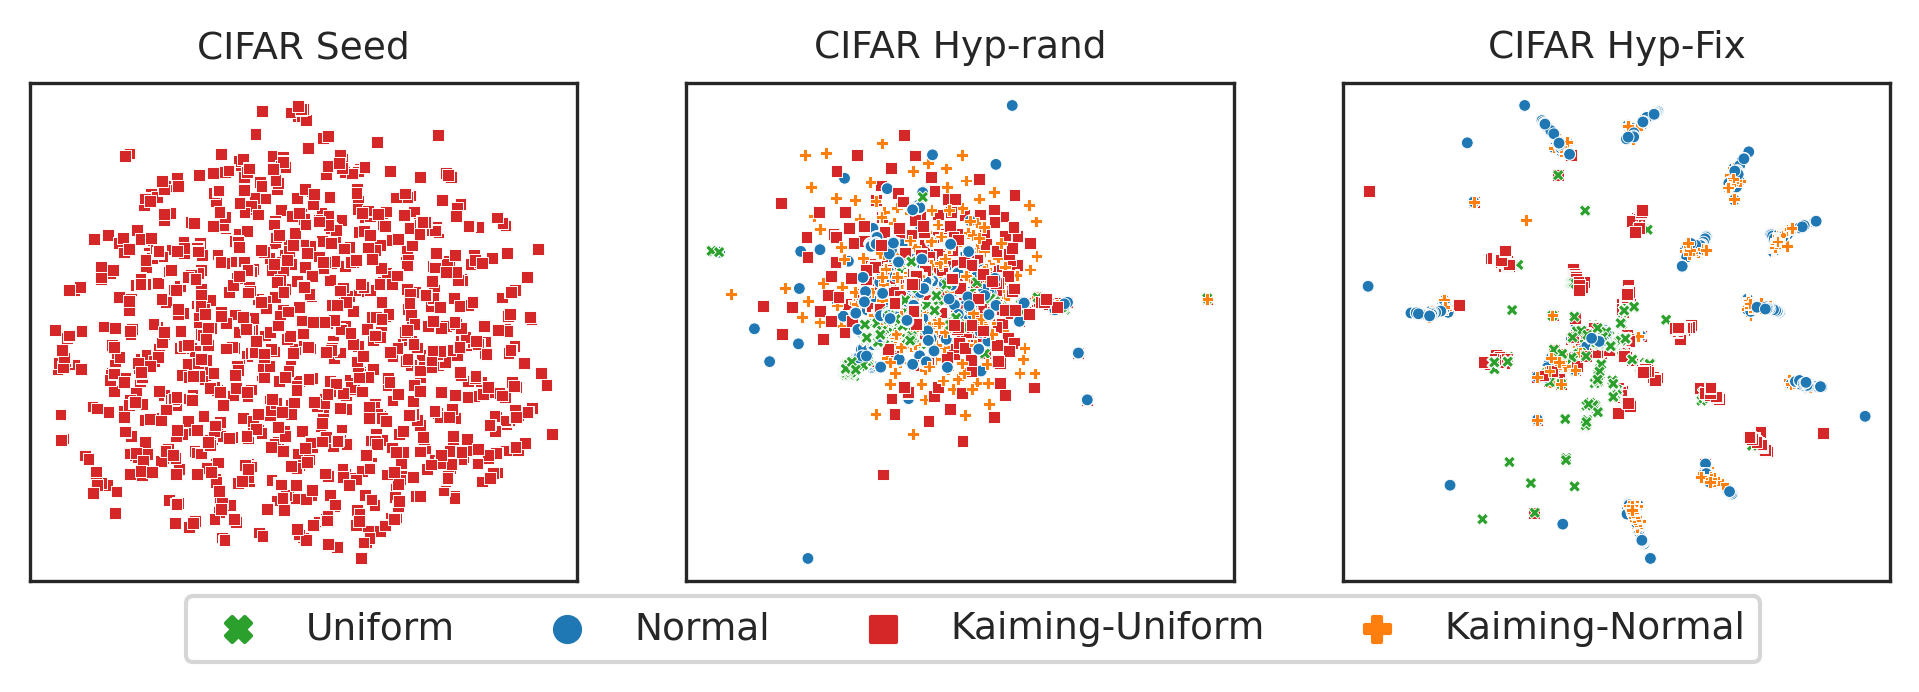
\includegraphics[trim=0in 0in 0in 0in, width=0.85\linewidth]{imgs/umap_visuals.png}
\vspace{-6pt}
\caption{
Visualization of the weights of the large CIFAR model zoos in different configurations. The weights are reduced to 2d using UMAP, preserving both local and global structure.
In the \texttt{Seed} configuration, the UMAP reduction contains little structure. The \texttt{Hyp-rand} is equally little structured.
In contrast, \texttt{Hyp-fix} contains visible clusters of initialization methods.\looseness-1
}
\vspace{-8pt}
\label{fig:umap_visualizations}    
\end{center}
\end{minipage}
\end{figure}
Lastly, we investigate the diversity of the model zoos in weight space, see again Table \ref{tab:analysis}. 
By design, the mean weight value of the zoos varying only in the seed is larger than in the other zoos, while the standard deviation does not differ greatly (Table \ref{tab:analysis}, column w). 
%%
To get a better intuition in the distribution of models in weight space, we compute the pairwise $\ell_2(\mathbf{w_k},\mathbf{w_l})=\frac{\|\mathbf{w_k}-\mathbf{w_l}\|_2^2}{1/N \sum_{n=1}^N\| \mathbf{w_n} \|_2^2}$ and cosine distance $cos(\mathbf{w_k},\mathbf{w_l}) = 1 - \frac{\mathbf{w_l}^T \mathbf{w_k}}{\|\mathbf{w_k}\|_2^2 \| \mathbf{w_l} \|_2^2}$, and investigate their distribution. 
Here, too, varying the hyperparameters introduces higher amounts of diversity, while changing or fixing the seeds does not affect the weight diversity much. As these values are computed at the end of model training, repeated starting points due to fixed seeds appear not to reduce weight diversity significantly.
%%
In a more hands-off approach, we compute 2d reductions of the weight over all epochs using UMAP ~\citep{mcinnesUMAPUniformManifold2018a}. 
In the 2d reductions (see Figure \ref{fig:umap_visualizations}), the zoos varying in seed only show little to no structure. Zoos with hyperparameter changes and random seeds are similarly unstructured. Zoos with varying hyperparameters and fixed seeds show clear clusters with models of the same initialization method and activation function. These findings are further supported by the predictability of initialization method and activation function (Table \ref{tab:benchmark_prediction}). The structures are unsurprising considering that the activation function is very influential in shaping the loss surface, while initialization method and the seed determine the starting point on it. Depending on the downstream task, this property can be desirable or should be avoided, which is why we provide both configurations.

\paragraph{Model Property Prediction}
As a set of benchmark results on the proposed model zoos and to further evaluate the zoos, we use linear models to predict hyperparameters or performance values of the individual models. 
As features, we use the model weights $\mathbf{w}$ or per-layer quintiles of the weights $s(\mathbf{w})$ as in~\citep{unterthinerPredictingNeuralNetwork2020}.
Linear models are used to evaluate the properties of the dataset and the quality of the features.
We report these results in Table \ref{tab:benchmark_prediction}.
The layer-wise weight statistics ($s(\mathbf{w})$) have generally higher predictive performance than the raw weights $\mathbf{w}$. 
In particular, $s(\mathbf{w})$ are not affected by using fixed or random seeds and thus generalize well to unseen seeds.
For the ResNet-18 zoos, $\mathbf{w}$ becomes too large to be used as a feature and is therefore omitted.
Across all zoos, the accuracy as well as the hyperparameters can be predicted very accurately. 
Generalization gap and epoch appear to be more difficult to predict. 
These findings hold for all zoos, regardless of the different architectures, model sizes, task complexity and performance range.
$\mathbf{w}$ can be used to predict the initialization method and activation function to very high accuracy, if the seeds are fixed. The performance drops drastically if seeds are varied. This results confirms our expectation of diversity in weight space induced by fixing or varying seed.
These results show i) that the model weights of our zoos contain rich information on their properties; ii) confirm the notions of diversity that were design goals for the zoos; and iii) leave room for improvements on the more difficult properties to predict, in particular the generalization gap.\looseness-1

%\todo{rm LR, cluster R^2 / accuracy. mark with stars}
\begin{table}[]
{
\scriptsize
\caption{Benchmark results for predicting model properties from the weights 
($\mathbf{w}$) and layer-wise weight statistics ($s(\mathbf{w})$) using linear models. 
We report the prediction $R^2$ for accuracy, generalization gap (GGap), epoch, learning rate (LR) and dropout (Drop) and prediction accuracy for initalization method (Init) and activation function (Act). 
Values reported in \%, higher values are better.
}
\label{tab:benchmark_prediction}
}
\begin{minipage}{\linewidth}
{
\scriptsize

% \begin{tabularx}{\linewidth}{lcXcccccccccc}
% \begin{tabular}{@{}llcccccccccccc@{}}
% >{\centering}
% \begin{tabular}{@{}p{0.06\textwidth}p{0.07\textwidth}p{0.04\textwidth}p{0.04\textwidth}p{0.04\textwidth}p{0.04\textwidth}p{0.04\textwidth}p{0.04\textwidth}p{0.04\textwidth}p{0.04\textwidth}p{0.04\textwidth}p{0.04\textwidth}p{0.04\textwidth}p{0.04\textwidth}@{}}
\begin{tabular}{
% @{}
    p{0.09\textwidth}
    p{0.08\textwidth}
    p{0.07\textwidth}
    >{\centering}p{0.037\textwidth}
    >{\centering}p{0.037\textwidth}
    >{\centering}p{0.037\textwidth}
    >{\centering}p{0.037\textwidth}
    >{\centering}p{0.037\textwidth}
    >{\centering}p{0.037\textwidth}
    >{\centering}p{0.037\textwidth}
    >{\centering}p{0.037\textwidth}
    >{\centering}p{0.037\textwidth}
    % >{\centering}p{0.037\textwidth}
    % >{\centering}p{0.037\textwidth}
    >{\centering\arraybackslash}p{0.037\textwidth}
    % @{}
    }

\toprule
                               & &               & \multicolumn{2}{c}{Accuracy} & \multicolumn{2}{c}{GGap} & \multicolumn{2}{c}{Epoch} & \multicolumn{2}{c}{Init} & \multicolumn{2}{c}{Act} \\ %& \multicolumn{2}{c}{Drop} \\
\cmidrule(rl){4-5} \cmidrule(rl){6-7} \cmidrule(rl){8-9} \cmidrule(rl){10-11} \cmidrule(rl){12-13} %\cmidrule(rl){14-15}
Dataset                       & Architecture        & Config & $\mathbf{w}$               & $s(\mathbf{w})$         & $\mathbf{w}$             & $s(\mathbf{w})$       & $\mathbf{w}$             & $s(\mathbf{w})$        & $\mathbf{w}$            & $s(\mathbf{w})$        & $\mathbf{w}$           & $s(\mathbf{w})$        \\%& $\mathbf{w}$             & $s(\mathbf{w})$       \\
\cmidrule(rl){1-1} \cmidrule(rl){2-2} \cmidrule(rl){3-3} \cmidrule(rl){4-5} \cmidrule(rl){6-7} \cmidrule(rl){8-9} \cmidrule(rl){10-11} \cmidrule(rl){12-13} %\cmidrule(rl){14-15}
\multirow{3}{*}{MNIST}         & CNN (s) & Seed          & 92.3           & 98.7        & 2.1          & 68.8      & 87.2         & 97.8       & n/a            & n/a           &     n/a       &  n/a          \\%&              &           \\
                               & CNN (s) & Hyp-10-r   & -11.2          & 69.4        & -49.8        & 13.7      & -95.5        & 14.3       & 42.6        & 77.6       & 45.5       & 78.5       \\%& -29.1        & 51.1      \\
                               & CNN (s) & Hyp-10-f    & 66.5           & 70.1        & 5.4          & 12.5      & -4.8         & 14.5       & 94.3        & 79.8       & 81.2       & 76.8       \\%& 64.2         & 57.1      \\
\cmidrule(rl){1-1} \cmidrule(rl){2-2} \cmidrule(rl){3-3} \cmidrule(rl){4-5} \cmidrule(rl){6-7} \cmidrule(rl){8-9} \cmidrule(rl){10-11} \cmidrule(rl){12-13} %\cmidrule(rl){14-15}
\multirow{3}{*}{F-MNIST}       & CNN (s) & Seed          & 87.5           & 97.2        & 20.9         & 60.5      & 89.1         & 97.1       &      n/a       &      n/a      &      n/a      &   n/a        \\% &              &           \\
                              & CNN (s) & Hyp-10-r   & 8.7            & 76.9        & -47.5        & 13.7      & -70.1        & 18.9       & 48.4        & 81.5       & 47.9       & 79.6      \\% & -16.7        & 56.5      \\
                              & CNN (s) & Hyp-10-f    & 62.4           & 75.6        & 3.9          & 12.6      & -2.0        & 17.0         & 95.4        & 81.6       & 84.6       & 77.7      \\% & 61           & 60.1      \\
\cmidrule(rl){1-1} \cmidrule(rl){2-2} \cmidrule(rl){3-3} \cmidrule(rl){4-5} \cmidrule(rl){6-7} \cmidrule(rl){8-9} \cmidrule(rl){10-11} \cmidrule(rl){12-13} %\cmidrule(rl){14-15}
\multirow{3}{*}{SVHN}          & CNN (s) & Seed          & 91.0             & 98.6        & -42.8        & 65.9      & 66.9         & 92.5       &   n/a          &      n/a      &     n/a       &   n/a        \\% &              &           \\
                              & CNN (s) & Hyp-10-r   & -8.6           & 90.3        & -55.3        & 27.6      & -30.5        & 11.1       & 38.2        & 58.5       & 55.7       & 72.3       \\%& -47.9        & 24.3      \\
                              & CNN (s) & Hyp-10-f    & 64.2           & 89.9        & 17.5         & 27.4      & -0.1         & 11.1       & 67.3        & 58.2       & 76.1       & 73.6      \\% & 30.2         & 30.7      \\
\cmidrule(rl){1-1} \cmidrule(rl){2-2} \cmidrule(rl){3-3} \cmidrule(rl){4-5} \cmidrule(rl){6-7} \cmidrule(rl){8-9} \cmidrule(rl){10-11} \cmidrule(rl){12-13} %\cmidrule(rl){14-15}
\multirow{3}{*}{USPS}          & CNN (s) & Seed          & 92.5           & 98.7        & 44.3         & 71.8      & 86.0         & 98.4       &     n/a        &    n/a        &       n/a     &    n/a       \\% &              &           \\
                              & CNN (s) & Hyp-10-r   & -11.5          & 70.3        & -35.2        & 13.6      & -75.7        & 21.3       & 49.2        & 88.8       & 43.7       & 66.2      \\% & -70.7        & 47        \\
                              & CNN (s) & Hyp-10-f    & 73.2           & 70.8        & 10.8         & 14.7      & 18.9         & 23.0         & 96.3        & 88.1       & 74.5       & 72.7       \\%& 59.6         & 48.2      \\
\cmidrule(rl){1-1} \cmidrule(rl){2-2} \cmidrule(rl){3-3} \cmidrule(rl){4-5} \cmidrule(rl){6-7} \cmidrule(rl){8-9} \cmidrule(rl){10-11} \cmidrule(rl){12-13} %\cmidrule(rl){14-15}
\multirow{3}{*}{CIFAR10} & CNN (s) & Seed          & 75.3           & 96.0          & 27.0           & 90.2      & 68.6         & 91.1       &     n/a        &        n/a    &    n/a        &   n/a        \\% &              &           \\
                              & CNN (s) & Hyp-10-r   & 50.1           & 88.0          & -4.3         & 40.5      & -2.7         & 34.2       & 34.0          & 50.5       & 71.5       & 80.9       \\%& 12.6         & 47.9      \\
                              & CNN (s) & Hyp-10-f    & 67.0             & 87.9        & 38.2         & 42.9      & 27.0           & 31.8       & 72.0          & 52.2       & 75.6       & 80.0        \\% & 37.6         & 41.5      \\
\cmidrule(rl){1-1} \cmidrule(rl){2-2} \cmidrule(rl){3-3} \cmidrule(rl){4-5} \cmidrule(rl){6-7} \cmidrule(rl){8-9} \cmidrule(rl){10-11} \cmidrule(rl){12-13} %\cmidrule(rl){14-15}

\multirow{3}{*}{CIFAR10} & CNN (l) & Seed          & 83.6           & 98.2        & 33.4         & 92.9      & 86.5         & 95.7       &     n/a        &        n/a    &  n/a          &       n/a    \\% &              &           \\
                              & CNN (l) & Hyp-10-r   & 32.6           & 90.5        & -0.9         & 47        & -10.5        & 35.5       & 41.6        & 51.6       & 69.1       & 83.1     \\%  & 2.8          & 57.8      \\
                              & CNN (l) & Hyp-10-f    & 64.5           & 91.4        & 30.4         & 40.7      & 29.8         & 35.3       & 74.5        & 54.9       & 77.7       & 86.0       \\%  & 40.8         & 51.2      \\
\cmidrule(rl){1-1} \cmidrule(rl){2-2} \cmidrule(rl){3-3} \cmidrule(rl){4-5} \cmidrule(rl){6-7} \cmidrule(rl){8-9} \cmidrule(rl){10-11} \cmidrule(rl){12-13} %\cmidrule(rl){14-15}
\multirow{3}{*}{STL}   & CNN (s) & Seed          & 17.8           & 91.2        & 2.0            & 30.2      & 45.3         & 95.0         &      n/a       &       n/a     &    n/a        &     n/a      \\% &              &           \\
                              & CNN (s) & Hyp-10-r   & -8.7           & 77.1        & -44.0          & 9.3       & -68.8        & 19.1       & 41.3        & 93.9       & 46.3       & 66.8     \\%  & -144       & 36.5      \\
                              & CNN (s) & Hyp-10-f    & 76.1           & 76.5        & 6.7          & 10.7      & 21.2         & 22.4       & 98.1        & 91.3       & 78.1       & 62.6      \\% & 51.1         & 48.5      \\
\cmidrule(rl){1-1} \cmidrule(rl){2-2} \cmidrule(rl){3-3} \cmidrule(rl){4-5} \cmidrule(rl){6-7} \cmidrule(rl){8-9} \cmidrule(rl){10-11} \cmidrule(rl){12-13} %\cmidrule(rl){14-15}
\multirow{3}{*}{STL}       & CNN (l) & Seed          & -112         & 94.2        & 2.8          & 37.3      & 5.6          & 98.7       &        n/a     &      n/a      &      n/a      &   n/a        \\% &              &           \\
                              & CNN (l) & Hyp-10-r      & -79.6          & 74.1        & -118       & 10.7      & -106         & 18.8       & 43.8        & 90.4       & 49.4       & 68.3     \\%  & -87.2        & 44.9      \\
                              & CNN (l) & Hyp-10-f      & 84.1           & 77.7        & 10.4         & 11.7      & 14.6         & 19.1       & 97.8        & 92.8       & 78.8       & 68.0      \\%   & 60.3         & 49.6      \\ 
\cmidrule(rl){1-1} \cmidrule(rl){2-2} \cmidrule(rl){3-3} \cmidrule(rl){4-5} \cmidrule(rl){6-7} \cmidrule(rl){8-9} \cmidrule(rl){10-11} \cmidrule(rl){12-13} %\cmidrule(rl){14-15}
CIFAR10                       & ResNet-18 & Seed          & --.- & 96.8 & --.- & 76.7 & --.- & 99.6 & n/a & n/a & n/a & n/a\\% &  &  \\
CIFAR100                      & ResNet-18 & Seed          & --.- & 97.4 & --.- & 95.4 & --.- & 99.9 & n/a & n/a & n/a & n/a\\% &  &  \\
t-ImageNet                    & ResNet-18 & Seed          & --.- & 96.1 & --.- & 87.5 & --.- & 99.9 & n/a & n/a & n/a & n/a\\% &  &  \\
\bottomrule
\end{tabular}
}
\vspace{-2mm}
\end{minipage}
\end{table}

